\documentclass[11pt,a4paper]{article}
\usepackage[margin=1in]{geometry}
\usepackage{amsmath}
\usepackage{amssymb}
\usepackage{titlesec}
\usepackage{enumitem}
\usepackage{xcolor}
\usepackage[most]{tcolorbox}
\usepackage{fancyhdr}
\usepackage{listings}
\usepackage{colortbl}
\usepackage{hyperref}
\usepackage{graphicx}
\usepackage{tikz}
\usepackage{mdframed}

% Color definitions
\definecolor{primaryblue}{RGB}{41, 128, 185}
\definecolor{secondaryblue}{RGB}{52, 152, 219}
\definecolor{darkgray}{RGB}{44, 62, 80}
\definecolor{lightgray}{RGB}{236, 240, 241}
\definecolor{codegreen}{RGB}{46, 204, 113}
\definecolor{codepurple}{RGB}{155, 89, 182}
\definecolor{codeorange}{RGB}{230, 126, 34}
\definecolor{codered}{RGB}{231, 76, 60}

\setlength{\headheight}{14pt}

% Header and Footer
\pagestyle{fancy}
\fancyhf{}
\lhead{\textcolor{primaryblue}{\textbf{DVC Pipeline Configuration}}}
\rhead{\textcolor{darkgray}{Complete Reference}}
\cfoot{\thepage}
\renewcommand{\headrulewidth}{0.5pt}
\renewcommand{\footrulewidth}{0.5pt}

% Title formatting
\titleformat{\section}
  {\LARGE\bfseries\color{primaryblue}}
  {\thesection}{1em}{}[\titlerule]

\titleformat{\subsection}
  {\Large\bfseries\color{secondaryblue}}
  {\thesubsection}{1em}{}

\titleformat{\subsubsection}
  {\large\bfseries\color{darkgray}}
  {\thesubsubsection}{1em}{}

% Code styling
\lstdefinelanguage{yaml}{
    keywords={true,false,null,y,n,yes,no},
    keywordstyle=\color{primaryblue}\bfseries,
    basicstyle=\ttfamily\small,
    sensitive=false,
    comment=[l]{\#},
    commentstyle=\color{codegreen}\ttfamily,
    stringstyle=\color{codered}\ttfamily,
    moredelim=[l][\color{codeorange}]{\&},
    moredelim=[l][\color{codepurple}]{*},
    morestring=[b]',
    morestring=[b]",
    literate={\ \ }{{\ }}1
}

\lstdefinelanguage{json}{
    string=[s]{"}{"},
    stringstyle=\color{codered},
    comment=[l]{//},
    commentstyle=\color{codegreen},
    morecomment=[s]{/*}{*/},
}

\lstset{
    backgroundcolor=\color{lightgray},
    basicstyle=\ttfamily\small,
    breaklines=true,
    frame=single,
    rulecolor=\color{darkgray},
    numbers=left,
    numberstyle=\tiny\color{darkgray},
    xleftmargin=2em,
    framexleftmargin=1.5em,
    showstringspaces=false,
    columns=flexible
}

% Custom boxes
\newtcolorbox{notebox}{
    colback=blue!5,
    colframe=primaryblue,
    boxrule=1pt,
    arc=3pt,
    left=5pt,
    right=5pt,
    top=5pt,
    bottom=5pt,
    breakable,
    enhanced jigsaw
}

\newtcolorbox{warningbox}{
    colback=yellow!10,
    colframe=codeorange,
    boxrule=1pt,
    arc=3pt,
    left=5pt,
    right=5pt,
    top=5pt,
    bottom=5pt,
    breakable,
    enhanced jigsaw
}

\newtcolorbox{tipbox}{
    colback=green!5,
    colframe=codegreen,
    boxrule=1pt,
    arc=3pt,
    left=5pt,
    right=5pt,
    top=5pt,
    bottom=5pt,
    breakable,
    enhanced jigsaw
}

\newtcolorbox{cmdbox}{
    colback=darkgray!5,
    colframe=darkgray,
    boxrule=1pt,
    arc=2pt,
    left=3pt,
    right=3pt,
    top=3pt,
    bottom=3pt,
    breakable,
    enhanced jigsaw
}

\begin{document}

% Title Page
\begin{titlepage}
    \centering
    \vspace*{1.5cm}
    
    {\Huge\bfseries\color{primaryblue} Data Version Control\par}
    \vspace{0.5cm}
    {\LARGE\color{secondaryblue} DVC Pipeline Configuration Guide\par}
    \vspace{2cm}
    
    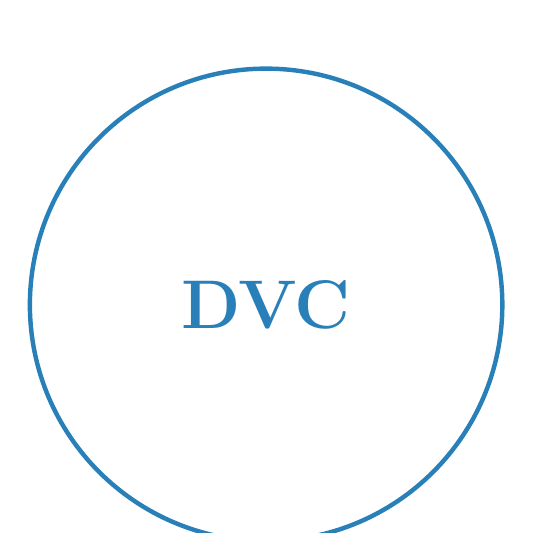
\begin{tikzpicture}
        \draw[primaryblue, ultra thick] (0,0) circle (3cm);
        \node at (0,0) {\Huge\bfseries\color{primaryblue} DVC};
    \end{tikzpicture}
    
    \vspace{2cm}
    {\Large Complete Reference for ML Pipeline Automation\par}
    \vspace{0.5cm}
    {\large Version Control for Data \& Models\par}
    
    \vfill
    
    {\Large\bfseries Sujil S\par}
    \vspace{0.3cm}
    {\large\texttt{sujil9480@gmail.com}\par}
    \vspace{1cm}
    {\large \today\par}
\end{titlepage}

\tableofcontents
\newpage

% ========================
% SECTION 1: INTRODUCTION
% ========================
\section{Introduction to DVC}

\subsection{What is DVC?}

\begin{notebox}
\textbf{DVC (Data Version Control)} is an open-source version control system for machine learning projects that extends Git's capabilities to handle large datasets, models, and ML workflows.
\end{notebox}

\subsubsection{Core Features}

\begin{itemize}[leftmargin=*]
    \item \textbf{Large File Management}: Efficiently version datasets $>$100MB
    \item \textbf{Pipeline Automation}: Reproducible ML workflows
    \item \textbf{Experiment Tracking}: Compare metrics and parameters
    \item \textbf{Model Versioning}: Track model evolution over time
    \item \textbf{Remote Storage}: Works with S3, GCS, Azure, SSH
    \item \textbf{Git Integration}: Seamless integration with Git workflow
\end{itemize}

\subsection{Why Use DVC?}

\subsubsection{Traditional Git Limitations}

\begin{warningbox}
\textbf{Problems with Git for ML Projects:}
\begin{itemize}[leftmargin=*]
    \item Cannot handle files $>$100MB efficiently
    \item Not optimized for binary files (models, datasets)
    \item No built-in experiment tracking
    \item Lacks pipeline automation
    \item Difficult to reproduce ML experiments
    \item Poor performance with large repositories
\end{itemize}
\end{warningbox}

\subsubsection{DVC Solutions}

\begin{tipbox}
\textbf{How DVC Solves These Problems:}
\begin{itemize}[leftmargin=*]
    \item \textbf{Efficient Storage}: Links to large files without storing in Git
    \item \textbf{Pipeline Automation}: Define workflows with \texttt{dvc.yaml}
    \item \textbf{Experiment Tracking}: Built-in metrics and parameter comparison
    \item \textbf{Reproducibility}: Guaranteed consistent results with \texttt{dvc.lock}
    \item \textbf{Collaboration}: Share data seamlessly via remote storage
    \item \textbf{Storage Agnostic}: Compatible with any cloud provider
\end{itemize}
\end{tipbox}

\subsection{DVC Architecture}

\subsubsection{Core Components}

\begin{enumerate}[leftmargin=*]
    \item \textbf{.dvc files}: Lightweight pointers to actual data
    \item \textbf{dvc.yaml}: Pipeline definition and stage configuration
    \item \textbf{dvc.lock}: Lock file with checksums for reproducibility
    \item \textbf{params.yaml}: Centralized parameter management
    \item \textbf{metrics/}: JSON/YAML files with evaluation metrics
    \item \textbf{.dvc/cache}: Local cache for tracked files
    \item \textbf{Remote Storage}: Cloud storage for team collaboration
\end{enumerate}

\subsubsection{Workflow Comparison}

\begin{center}
\begin{tabular}{|p{0.45\textwidth}|p{0.45\textwidth}|}
\hline
\rowcolor{primaryblue!20}
\textbf{Git Workflow} & \textbf{DVC Workflow} \\
\hline
Tracks source code & Tracks data and models \\
\hline
Optimized for text files & Optimized for large binary files \\
\hline
Stores in \texttt{.git/} directory & Stores in \texttt{.dvc/cache} \\
\hline
\texttt{git commit, push, pull} & \texttt{dvc add, push, pull} \\
\hline
Remote: GitHub, GitLab & Remote: S3, GCS, Azure \\
\hline
Files tracked directly & Files tracked via pointers \\
\hline
\end{tabular}
\end{center}

\subsection{Getting Started}

\subsubsection{Installation}

\begin{cmdbox}
\begin{verbatim}
# Install DVC with pip
pip install dvc

# Install with specific remote support
pip install dvc[s3]      # AWS S3
pip install dvc[gs]      # Google Cloud Storage
pip install dvc[azure]   # Azure Blob Storage
pip install dvc[ssh]     # SSH remote
pip install dvc[all]     # All remotes

# Verify installation
dvc version
\end{verbatim}
\end{cmdbox}

\subsubsection{Project Initialization}

\begin{cmdbox}
\begin{verbatim}
# Initialize Git repository
git init

# Initialize DVC
dvc init

# Commit DVC configuration
git add .dvc .gitignore
git commit -m "Initialize DVC"
\end{verbatim}
\end{cmdbox}

\newpage

% ========================
% SECTION 2: DVC.YAML
% ========================
\section{Understanding dvc.yaml}

\subsection{What is dvc.yaml?}

\begin{notebox}
\textbf{dvc.yaml} is the central pipeline configuration file that defines your entire ML workflow. It describes stages, dependencies, commands, outputs, parameters, and metrics in a declarative YAML format.
\end{notebox}

\subsection{Basic Structure}

\subsubsection{Minimal Pipeline}

\begin{lstlisting}[language=yaml]
stages:
  stage_name:
    cmd: python script.py
    deps:
      - input_file.csv
    outs:
      - output_file.csv
\end{lstlisting}

\subsubsection{Complete Stage Definition}

\begin{lstlisting}[language=yaml]
stages:
  training:
    cmd: python train.py --epochs 100
    wdir: src/                        # Working directory
    deps:
      - data/processed/train.csv      # Data dependencies
      - src/train.py                  # Code dependencies
      - src/models/architecture.py    # Module dependencies
    params:
      - training.learning_rate        # Parameter references
      - training.batch_size
      - model.architecture
    outs:
      - models/model.pkl              # Model outputs
      - models/weights.h5
    metrics:
      - metrics/scores.json:          # Metrics (not cached)
          cache: false
    plots:
      - plots/training_curve.csv:     # Plot data
          cache: false
          x: epoch
          y: loss
    frozen: false                     # Allow automatic execution
\end{lstlisting}

\subsection{Key Benefits}

\begin{tipbox}
\textbf{Why Use dvc.yaml?}
\begin{itemize}[leftmargin=*]
    \item \textbf{Reproducibility}: Execute exact same workflow every time
    \item \textbf{Automation}: Run entire pipeline with single command
    \item \textbf{Dependency Tracking}: Only re-run stages with changes
    \item \textbf{Version Control}: Track pipeline evolution in Git
    \item \textbf{Documentation}: Self-documenting workflow
    \item \textbf{Collaboration}: Share workflows with team members
\end{itemize}
\end{tipbox}

\newpage

% ========================
% SECTION 3: CORE COMPONENTS
% ========================
\section{Core Components}

\subsection{Stages}

\textbf{Stages} are the fundamental building blocks representing discrete steps in your ML pipeline.

\subsubsection{Stage Characteristics}

\begin{itemize}[leftmargin=*]
    \item Each stage has a unique identifier name
    \item Stages execute in dependency order (DAG)
    \item Outputs are cached to avoid redundant computation
    \item Changes in dependencies trigger re-execution
    \item Multiple stages can run in parallel if independent
\end{itemize}

\subsubsection{Simple Stage Example}

\begin{lstlisting}[language=yaml]
stages:
  preprocess:
    cmd: python src/preprocess.py
    deps:
      - data/raw/dataset.csv
      - src/preprocess.py
    outs:
      - data/processed/train.csv
      - data/processed/test.csv
\end{lstlisting}

\subsection{Commands (cmd)}

The \textbf{cmd} field specifies the shell command to execute.

\subsubsection{Command Variations}

\begin{lstlisting}[language=yaml]
# Simple command
stages:
  train:
    cmd: python train.py

# Command with arguments
stages:
  train:
    cmd: python train.py --epochs 100 --lr 0.001

# Multi-line command
stages:
  pipeline:
    cmd: >
      python preprocess.py &&
      python train.py &&
      python evaluate.py

# Command with environment variables
stages:
  gpu_train:
    cmd: CUDA_VISIBLE_DEVICES=0 python train.py

# Command with shell features
stages:
  batch_process:
    cmd: for file in data/*.csv; do python process.py $file; done
\end{lstlisting}

\subsection{Dependencies (deps)}

\textbf{Dependencies} are files or directories that trigger stage re-execution when modified.

\subsubsection{Dependency Types}

\begin{lstlisting}[language=yaml]
stages:
  train:
    cmd: python train.py
    deps:
      # Data dependencies
      - data/processed/train.csv
      - data/processed/validation.csv
      
      # Code dependencies
      - src/train.py
      - src/models/neural_network.py
      - src/utils/data_loader.py
      
      # Configuration files
      - configs/model_config.yaml
      
      # Pre-trained models
      - models/pretrained/base_model.pkl
      
      # Directory dependencies
      - data/images/
\end{lstlisting}

\begin{warningbox}
\textbf{Important}: Always include ALL files that affect stage output. Missing dependencies can lead to inconsistent results and break reproducibility.
\end{warningbox}

\subsection{Outputs (outs)}

\textbf{Outputs} are files or directories produced by a stage.

\subsubsection{Output Configuration}

\begin{lstlisting}[language=yaml]
stages:
  train:
    cmd: python train.py
    outs:
      # Simple outputs (cached by default)
      - models/model.pkl
      - models/weights.h5
      
      # Outputs with custom settings
      - models/final_model.pkl:
          cache: true               # Cache this output
          persist: false            # Remove when not current
      
      - logs/training.log:
          cache: false              # Don't cache logs
      
      - checkpoints/:
          cache: true
          persist: true             # Keep even when not current
\end{lstlisting}

\subsubsection{Output Options}

\begin{center}
\begin{tabular}{|l|p{0.6\textwidth}|}
\hline
\rowcolor{primaryblue!20}
\textbf{Option} & \textbf{Description} \\
\hline
\texttt{cache} & Cache output (default: \texttt{true}) \\
\hline
\texttt{persist} & Keep in workspace when not current (default: \texttt{false}) \\
\hline
\texttt{checkpoint} & Mark as ML checkpoint for experiments \\
\hline
\texttt{desc} & Human-readable description \\
\hline
\end{tabular}
\end{center}

\subsection{Parameters (params)}

\textbf{Parameters} reference values from external files (typically \texttt{params.yaml}).

\subsubsection{Parameter Usage}

\begin{lstlisting}[language=yaml]
# dvc.yaml
stages:
  train:
    cmd: python train.py
    params:
      - training.epochs              # Specific parameter
      - training.learning_rate
      - training.batch_size
      - model                        # Entire section
      - optimizer.type
      - optimizer.beta1
\end{lstlisting}

\begin{lstlisting}[language=yaml]
# params.yaml
training:
  epochs: 100
  learning_rate: 0.001
  batch_size: 32
  early_stopping: true

model:
  architecture: resnet50
  layers: 18
  dropout: 0.5
  activation: relu

optimizer:
  type: adam
  beta1: 0.9
  beta2: 0.999
\end{lstlisting}

\subsubsection{Multiple Parameter Files}

\begin{lstlisting}[language=yaml]
stages:
  train:
    cmd: python train.py
    params:
      - params.yaml:
          - training
          - model
      - configs/advanced.yaml:
          - augmentation
          - preprocessing
\end{lstlisting}

\subsection{Metrics}

\textbf{Metrics} are evaluation results stored in JSON, YAML, CSV, or TSV format.

\subsubsection{Metric Definition}

\begin{lstlisting}[language=yaml]
stages:
  evaluate:
    cmd: python evaluate.py
    deps:
      - data/test.csv
      - models/model.pkl
    metrics:
      - metrics/test_scores.json:
          cache: false              # NEVER cache metrics
      - metrics/confusion_matrix.json:
          cache: false
\end{lstlisting}

\subsubsection{Metric File Format}

\begin{lstlisting}[language=json]
{
  "accuracy": 0.9542,
  "precision": 0.9321,
  "recall": 0.9456,
  "f1_score": 0.9388,
  "auc_roc": 0.9782,
  "confusion_matrix": {
    "true_positive": 850,
    "false_positive": 45,
    "true_negative": 920,
    "false_negative": 35
  }
}
\end{lstlisting}

\subsubsection{Viewing Metrics}

\begin{cmdbox}
\begin{verbatim}
# Show current metrics
dvc metrics show

# Compare with another branch
dvc metrics diff main

# Compare with previous commit
dvc metrics diff HEAD~1

# Show all experiments
dvc metrics show -R
\end{verbatim}
\end{cmdbox}

\subsection{Plots}

\textbf{Plots} are data files for visualization (CSV, JSON, YAML).

\subsubsection{Plot Configuration}

\begin{lstlisting}[language=yaml]
stages:
  evaluate:
    cmd: python evaluate.py
    plots:
      # Simple plot
      - plots/training_history.csv:
          cache: false
      
      # Customized plot
      - plots/roc_curve.json:
          cache: false
          x: fpr
          y: tpr
          title: "ROC Curve"
          x_label: "False Positive Rate"
          y_label: "True Positive Rate"
      
      # Multi-series plot
      - plots/metrics.csv:
          x: epoch
          y:
            plots/metrics.csv: [loss, val_loss]
          title: "Training vs Validation Loss"
\end{lstlisting}

\subsubsection{Plot Data Format}

\begin{lstlisting}
# plots/training_history.csv
epoch,loss,accuracy,val_loss,val_accuracy
1,0.693,0.501,0.685,0.515
2,0.612,0.653,0.598,0.672
3,0.523,0.745,0.501,0.758
4,0.445,0.812,0.432,0.825
5,0.389,0.856,0.398,0.861
\end{lstlisting}

\newpage

% ========================
% SECTION 4: ADVANCED FEATURES
% ========================
\section{Advanced Pipeline Features}

\subsection{Working Directory (wdir)}

Execute stages in a specific working directory.

\begin{lstlisting}[language=yaml]
stages:
  notebook_analysis:
    cmd: jupyter nbconvert --execute analysis.ipynb
    wdir: notebooks/
    deps:
      - notebooks/analysis.ipynb
      - data/input.csv
    outs:
      - notebooks/output.html
      - notebooks/results.csv
\end{lstlisting}

\subsection{Frozen Stages}

Prevent automatic execution of specific stages.

\begin{lstlisting}[language=yaml]
stages:
  expensive_preprocessing:
    cmd: python expensive_process.py
    frozen: true                    # Skip in dvc repro
    deps:
      - data/raw/large_dataset.csv
    outs:
      - data/processed/features.pkl
\end{lstlisting}

\begin{tipbox}
\textbf{Use Cases for Frozen Stages:}
\begin{itemize}[leftmargin=*]
    \item Computationally expensive operations
    \item Stages requiring manual intervention
    \item Optional pipeline branches
    \item Data collection/download stages
\end{itemize}
\end{tipbox}

\subsection{Always Changed Stages}

Force re-execution regardless of dependencies.

\begin{lstlisting}[language=yaml]
stages:
  fetch_data:
    cmd: python fetch_latest_data.py
    always_changed: true            # Always runs
    outs:
      - data/latest/dataset.csv
      - data/latest/metadata.json
\end{lstlisting}

\subsection{Foreach Loops}

Execute the same stage multiple times with different parameters.

\subsubsection{Simple Foreach}

\begin{lstlisting}[language=yaml]
stages:
  train_models:
    foreach:
      - logistic_regression
      - random_forest
      - gradient_boosting
      - neural_network
      - svm
    do:
      cmd: python train.py --model ${item}
      deps:
        - data/train.csv
        - src/train.py
      params:
        - models.${item}
      outs:
        - models/${item}/model.pkl
      metrics:
        - metrics/${item}_scores.json:
            cache: false
\end{lstlisting}

\subsubsection{Dictionary Foreach}

\begin{lstlisting}[language=yaml]
stages:
  process_datasets:
    foreach:
      train: data/raw/train.csv
      validation: data/raw/val.csv
      test: data/raw/test.csv
    do:
      cmd: python process.py --input ${item} --output data/processed/${key}.csv
      deps:
        - ${item}
        - src/process.py
      outs:
        - data/processed/${key}.csv
\end{lstlisting}

\subsubsection{Matrix Foreach (Hyperparameter Grid)}

\begin{lstlisting}[language=yaml]
stages:
  grid_search:
    foreach:
      lr_0001_bs16:
        learning_rate: 0.001
        batch_size: 16
      lr_0001_bs32:
        learning_rate: 0.001
        batch_size: 32
      lr_001_bs16:
        learning_rate: 0.01
        batch_size: 16
      lr_001_bs32:
        learning_rate: 0.01
        batch_size: 32
    do:
      cmd: >
        python train.py 
        --lr ${item.learning_rate} 
        --batch ${item.batch_size}
      deps:
        - data/train.csv
      outs:
        - models/${key}_model.pkl
      metrics:
        - metrics/${key}_scores.json:
            cache: false
\end{lstlisting}

\subsection{Variables and Templating}

Define reusable variables for cleaner configuration.

\begin{lstlisting}[language=yaml]
vars:
  - base_dir: .
  - data_dir: data
  - models_dir: models
  - metrics_dir: metrics
  - src_dir: src
  - batch_size: 32
  - learning_rate: 0.001
  - random_seed: 42

stages:
  preprocess:
    cmd: python ${src_dir}/preprocess.py --seed ${random_seed}
    deps:
      - ${data_dir}/raw/dataset.csv
      - ${src_dir}/preprocess.py
    outs:
      - ${data_dir}/processed/train.csv
      - ${data_dir}/processed/test.csv
  
  train:
    cmd: >
      python ${src_dir}/train.py 
      --batch-size ${batch_size}
      --lr ${learning_rate}
      --seed ${random_seed}
    deps:
      - ${data_dir}/processed/train.csv
      - ${src_dir}/train.py
    outs:
      - ${models_dir}/model.pkl
    metrics:
      - ${metrics_dir}/scores.json:
          cache: false
\end{lstlisting}

\subsection{Stage Dependencies}

Explicitly define execution order (rarely needed).

\begin{lstlisting}[language=yaml]
stages:
  stage_a:
    cmd: python a.py
    outs:
      - output_a.csv
  
  stage_b:
    cmd: python b.py
    deps:
      - output_a.csv         # Implicit dependency on stage_a
    outs:
      - output_b.csv
  
  stage_c:
    cmd: python c.py
    deps:
      - output_b.csv         # Implicit dependency on stage_b
    outs:
      - output_c.csv
\end{lstlisting}

\begin{notebox}
\textbf{Note}: DVC automatically determines execution order from file dependencies. Explicit stage dependencies are rarely needed.
\end{notebox}

\newpage

% ========================
% SECTION 5: COMPLETE EXAMPLE
% ========================
\section{Complete ML Pipeline Example}

\subsection{Project Structure}

\begin{cmdbox}
\begin{verbatim}
ml_project/
|-- dvc.yaml
|-- params.yaml
|-- .dvc/
|   |-- config
|   `-- cache/
|-- data/
|   |-- raw/
|   |-- processed/
|   `-- features/
|-- models/
|-- metrics/
|-- plots/
|-- src/
|   |-- data_collection.py
|   |-- preprocessing.py
|   |-- feature_engineering.py
|   |-- train.py
|   |-- evaluate.py
|   `-- models/
|       `-- architectures.py
|-- notebooks/
|-- requirements.txt
`-- README.md
\end{verbatim}
\end{cmdbox}

\subsection{Complete dvc.yaml}

\begin{lstlisting}[language=yaml]
vars:
  - data_dir: data
  - models_dir: models
  - metrics_dir: metrics
  - plots_dir: plots
  - src_dir: src

stages:
  # ==========================================
  # Stage 1: Data Collection
  # ==========================================
  collect_data:
    cmd: python ${src_dir}/data_collection.py
    deps:
      - ${src_dir}/data_collection.py
    params:
      - data_collection.source_url
      - data_collection.date_range
      - data_collection.api_version
    outs:
      - ${data_dir}/raw/dataset.csv
      - ${data_dir}/raw/metadata.json

  # ==========================================
  # Stage 2: Data Preprocessing
  # ==========================================
  preprocess:
    cmd: python ${src_dir}/preprocessing.py
    deps:
      - ${data_dir}/raw/dataset.csv
      - ${src_dir}/preprocessing.py
    params:
      - preprocessing.train_split
      - preprocessing.test_split
      - preprocessing.validation_split
      - preprocessing.random_seed
      - preprocessing.handle_missing
      - preprocessing.remove_outliers
    outs:
      - ${data_dir}/processed/train.csv
      - ${data_dir}/processed/test.csv
      - ${data_dir}/processed/validation.csv
      - ${data_dir}/processed/stats.json

  # ==========================================
  # Stage 3: Feature Engineering
  # ==========================================
  feature_engineering:
    cmd: python ${src_dir}/feature_engineering.py
    deps:
      - ${data_dir}/processed/train.csv
      - ${data_dir}/processed/test.csv
      - ${data_dir}/processed/validation.csv
      - ${src_dir}/feature_engineering.py
    params:
      - features.numerical_features
      - features.categorical_features
      - features.text_features
      - features.scaling_method
      - features.encoding_method
    outs:
      - ${data_dir}/features/X_train.npy
      - ${data_dir}/features/X_test.npy
      - ${data_dir}/features/X_val.npy
      - ${data_dir}/features/y_train.npy
      - ${data_dir}/features/y_test.npy
      - ${data_dir}/features/y_val.npy
      - ${models_dir}/preprocessors/scaler.pkl
      - ${models_dir}/preprocessors/encoder.pkl

  # ==========================================
  # Stage 4: Model Training
  # ==========================================
  train:
    cmd: python ${src_dir}/train.py
    deps:
      - ${data_dir}/features/X_train.npy
      - ${data_dir}/features/X_val.npy
      - ${data_dir}/features/y_train.npy
      - ${data_dir}/features/y_val.npy
      - ${src_dir}/train.py
      - ${src_dir}/models/architectures.py
    params:
      - training.model_type
      - training.epochs
      - training.batch_size
      - training.learning_rate
      - training.optimizer
      - training.loss_function
      - training.early_stopping
      - training.random_seed
    outs:
      - ${models_dir}/trained/model.pkl
      - ${models_dir}/trained/weights.h5
      - ${models_dir}/trained/history.json
    plots:
      - ${plots_dir}/training_loss.csv:
          cache: false
          x: epoch
          y: [loss, val_loss]
          title: "Training vs Validation Loss"
      - ${plots_dir}/training_accuracy.csv:
          cache: false
          x: epoch
          y: [accuracy, val_accuracy]

  # ==========================================
  # Stage 5: Model Evaluation
  # ==========================================
  evaluate:
    cmd: python ${src_dir}/evaluate.py
    deps:
      - ${data_dir}/features/X_test.npy
      - ${data_dir}/features/y_test.npy
      - ${models_dir}/trained/model.pkl
      - ${models_dir}/preprocessors/scaler.pkl
      - ${src_dir}/evaluate.py
    params:
      - evaluation.metrics
      - evaluation.threshold
    outs:
      - predictions/test_predictions.csv
    metrics:
      - ${metrics_dir}/test_scores.json:
          cache: false
    plots:
      - ${plots_dir}/confusion_matrix.csv:
          cache: false
          template: confusion
      - ${plots_dir}/roc_curve.json:
          cache: false
          x: fpr
          y: tpr
          title: "ROC Curve"
      - ${plots_dir}/precision_recall.json:
          cache: false
          x: recall
          y: precision
\end{lstlisting}

\subsection{Complete params.yaml}

\begin{lstlisting}[language=yaml]
# ==========================================
# Data Collection Parameters
# ==========================================
data_collection:
  source_url: "https://api.example.com/v2/dataset"
  date_range:
    start: "2024-01-01"
    end: "2024-12-31"
  api_version: "v2.0"
  timeout: 30

# ==========================================
# Preprocessing Parameters
# ==========================================
preprocessing:
  train_split: 0.70
  test_split: 0.20
  validation_split: 0.10
  random_seed: 42
  handle_missing: "median"
  remove_outliers: true
  outlier_method: "iqr"
  outlier_threshold: 1.5

# ==========================================
# Feature Engineering
# ==========================================
features:
  numerical_features:
    - age
    - income
    - credit_score
    - balance
  
  categorical_features:
    - gender
    - occupation
    - education
  
  text_features:
    - description
  
  scaling_method: "standard"
  encoding_method: "onehot"

# ==========================================
# Training Parameters
# ==========================================
training:
  model_type: "random_forest"
  epochs: 100
  batch_size: 32
  learning_rate: 0.001
  optimizer: "adam"
  loss_function: "binary_crossentropy"
  early_stopping:
    enabled: true
    patience: 10
    min_delta: 0.001
  random_seed: 42

# ==========================================
# Evaluation Parameters
# ==========================================
evaluation:
  metrics:
    - accuracy
    - precision
    - recall
    - f1_score
    - roc_auc
  threshold: 0.5
\end{lstlisting}

\newpage

% ========================
% SECTION 6: DVC COMMANDS
% ========================
\section{Essential DVC Commands}

\subsection{Initialization and Setup}

\begin{cmdbox}
\begin{verbatim}
# Initialize DVC in project
dvc init

# Configure S3 remote
dvc remote add -d storage s3://mybucket/dvcstore

# Configure GCS remote
dvc remote add -d storage gs://mybucket/dvcstore

# List remotes
dvc remote list

# Modify remote URL
dvc remote modify storage url s3://newbucket/path
\end{verbatim}
\end{cmdbox}

\subsection{Pipeline Operations}

\begin{cmdbox}
\begin{verbatim}
# Run entire pipeline
dvc repro

# Run specific stage
dvc repro train

# Force re-run all stages
dvc repro -f

# Force re-run specific stage
dvc repro -f preprocess

# Show pipeline DAG
dvc dag

# Check pipeline status
dvc status

# Detailed status
dvc status -v
\end{verbatim}
\end{cmdbox}

\subsection{Data Management}

\begin{cmdbox}
\begin{verbatim}
# Track large file
dvc add data/dataset.csv

# Track directory
dvc add data/images/

# Push data to remote
dvc push

# Pull data from remote
dvc pull

# Fetch to cache only
dvc fetch

# Update workspace from cache
dvc checkout
\end{verbatim}
\end{cmdbox}

\subsection{Metrics and Plots}

\begin{cmdbox}
\begin{verbatim}
# Show metrics
dvc metrics show

# Compare metrics with branch
dvc metrics diff main

# Show plots
dvc plots show

# Compare plots
dvc plots diff main experiment

# Generate HTML report
dvc plots show --html
\end{verbatim}
\end{cmdbox}

\subsection{Experiments}

\begin{cmdbox}
\begin{verbatim}
# Run experiment
dvc exp run

# Run with parameter override
dvc exp run -S train.lr=0.01

# Queue experiments
dvc exp run --queue -S train.lr=0.001
dvc exp run --queue -S train.lr=0.01
dvc queue start

# List experiments
dvc exp show

# Compare experiments
dvc exp diff

# Apply experiment
dvc exp apply exp-12345
\end{verbatim}
\end{cmdbox}

\newpage

% ========================
% SECTION 7: BEST PRACTICES
% ========================
\section{Best Practices}

\subsection{Pipeline Design}

\begin{tipbox}
\textbf{Good Practices:}
\begin{itemize}[leftmargin=*]
    \item Create stages for logical workflow steps
    \item Keep stages focused (single responsibility)
    \item Use descriptive stage names (\texttt{preprocess\_data}, not \texttt{stage1})
    \item Track all dependencies accurately
    \item Organize outputs in structured directories
    \item Use \texttt{params.yaml} for all configurable values
\end{itemize}
\end{tipbox}

\begin{warningbox}
\textbf{Avoid:}
\begin{itemize}[leftmargin=*]
    \item Overly granular stages (creates overhead)
    \item Combining unrelated operations in one stage
    \item Missing dependencies (breaks reproducibility)
    \item Hardcoding parameters in commands
    \item Caching log files and metrics
\end{itemize}
\end{warningbox}

\subsection{Version Control Integration}

\subsubsection{Track with Git}

\begin{itemize}[leftmargin=*]
    \item \texttt{dvc.yaml} - Pipeline definition
    \item \texttt{dvc.lock} - Lock file
    \item \texttt{params.yaml} - Parameters
    \item \texttt{*.dvc} - File pointers
    \item \texttt{.dvc/config} - Configuration
    \item \texttt{src/} - Source code
\end{itemize}

\subsubsection{Track with DVC}

\begin{itemize}[leftmargin=*]
    \item \texttt{data/} - Datasets
    \item \texttt{models/} - Trained models
    \item Large files ($>$1MB)
\end{itemize}

\subsection{Parameter Management}

\begin{lstlisting}[language=yaml]
# Good: Hierarchical structure
preprocessing:
  train_split: 0.7
  random_seed: 42

training:
  epochs: 100
  learning_rate: 0.001

# Bad: Flat structure
train_split: 0.7
epochs: 100
learning_rate: 0.001
\end{lstlisting}

\newpage

% ========================
% SECTION 8: TROUBLESHOOTING
% ========================
\section{Troubleshooting}

\subsection{Pipeline Won't Run}

\textbf{Problem}: \texttt{dvc repro} doesn't execute stages

\vspace{0.5em}
\textbf{Possible Causes}:
\begin{itemize}[leftmargin=*]
    \item Pipeline already up-to-date (no changes detected)
    \item Syntax errors in \texttt{dvc.yaml}
    \item Missing dependencies
    \item Circular dependencies
    \item Frozen stages
\end{itemize}

\begin{cmdbox}
\begin{verbatim}
# Check pipeline status
dvc status
dvc status -v

# Validate pipeline structure
dvc dag

# Force re-run entire pipeline
dvc repro -f

# Force re-run specific stage
dvc repro -f stage_name

# Check for syntax errors
cat dvc.yaml | python -m yaml

# Dry run (show what would execute)
dvc repro --dry
\end{verbatim}
\end{cmdbox}

\subsection{Stage Always Re-runs}

\textbf{Problem}: Stage executes every time despite no changes

\vspace{0.5em}
\textbf{Possible Causes}:
\begin{itemize}[leftmargin=*]
    \item Missing dependencies in \texttt{deps} field
    \item Files being modified by external processes
    \item Non-deterministic code (random operations without seed)
    \item Timestamp issues
    \item Command generates different output each time
\end{itemize}

\textbf{Solutions}:

\begin{cmdbox}
\begin{verbatim}
# Check what DVC detects as changed
dvc status -v

# Verify file checksums
dvc status --show-json

# Set random seeds in your code
# Python example:
import random
import numpy as np
random.seed(42)
np.random.seed(42)
\end{verbatim}
\end{cmdbox}

\begin{tipbox}
\textbf{Ensure Reproducibility}:
\begin{itemize}[leftmargin=*]
    \item List ALL dependencies (data, code, configs)
    \item Set random seeds for all random operations
    \item Avoid timestamp-based operations
    \item Use deterministic algorithms
\end{itemize}
\end{tipbox}

\subsection{Missing Data Files}

\textbf{Problem}: Data files not found after cloning repository

\begin{cmdbox}
\begin{verbatim}
# Pull all data from remote
dvc pull

# Pull specific file
dvc pull data/dataset.csv.dvc

# Check remote configuration
dvc remote list
dvc remote list --show-origin

# Test connectivity to remote
dvc status --cloud

# Check if files are in cache
ls -la .dvc/cache/

# Fetch to cache without checking out
dvc fetch
dvc checkout
\end{verbatim}
\end{cmdbox}

\subsection{Push/Pull Failures}

\textbf{Problem}: Cannot push or pull data to/from remote

\vspace{0.5em}
\textbf{Common Issues}:
\begin{itemize}[leftmargin=*]
    \item Incorrect remote URL
    \item Missing credentials
    \item Permission issues
    \item Network connectivity
    \item Insufficient storage quota
\end{itemize}

\begin{cmdbox}
\begin{verbatim}
# Check remote configuration
dvc remote list
dvc config remote.storage.url

# Verbose output for debugging
dvc push -v
dvc pull -v

# Check cloud status
dvc status --cloud

# For AWS S3 - verify credentials
aws configure list
aws s3 ls s3://your-bucket/

# For Google Cloud - verify authentication
gcloud auth list
gsutil ls gs://your-bucket/

# Test with small file first
dvc add test.txt
dvc push test.txt.dvc
\end{verbatim}
\end{cmdbox}

\subsection{Cache Corruption}

\textbf{Problem}: DVC cache becomes corrupted or inconsistent

\begin{cmdbox}
\begin{verbatim}
# Check cache integrity
ls -la .dvc/cache/

# Remove corrupted cache
rm -rf .dvc/cache

# Re-download from remote
dvc fetch
dvc checkout

# Or re-run pipeline
dvc repro -f

# Verify data integrity
dvc status
\end{verbatim}
\end{cmdbox}

\subsection{Disk Space Issues}

\textbf{Problem}: DVC cache consuming too much disk space

\begin{cmdbox}
\begin{verbatim}
# Check cache size
du -sh .dvc/cache
dvc cache dir

# Show what would be removed (dry run)
dvc gc --dry

# Remove files not in current workspace
dvc gc --workspace

# Keep workspace, all branches, and all tags
dvc gc --workspace --all-branches --all-tags

# Remove all except workspace
dvc gc --workspace --force

# Clean cloud cache
dvc gc --cloud

# Check after cleanup
du -sh .dvc/cache
\end{verbatim}
\end{cmdbox}

\begin{warningbox}
\textbf{Warning}: Be careful with \texttt{dvc gc}. Always use \texttt{--dry} first to see what would be removed. Keep backups of important data.
\end{warningbox}

\subsection{Lock File Conflicts}

\textbf{Problem}: Git merge conflict in \texttt{dvc.lock}

\vspace{0.5em}
\textbf{Solution 1: Accept One Version}

\begin{cmdbox}
\begin{verbatim}
# Accept your version
git checkout --ours dvc.lock

# Or accept their version
git checkout --theirs dvc.lock

# Regenerate lock file
dvc repro

# Commit resolution
git add dvc.lock
git commit -m "Resolve dvc.lock conflict"
\end{verbatim}
\end{cmdbox}

\textbf{Solution 2: Regenerate}

\begin{cmdbox}
\begin{verbatim}
# Remove conflicted lock file
rm dvc.lock

# Regenerate from pipeline
dvc repro

# Commit new lock file
git add dvc.lock
git commit -m "Regenerate dvc.lock"
\end{verbatim}
\end{cmdbox}

\subsection{Permission Issues}

\textbf{Problem}: Permission denied errors

\begin{cmdbox}
\begin{verbatim}
# Fix local cache permissions
chmod -R u+w .dvc/cache

# Fix workspace file permissions
chmod -R u+w data/ models/

# For remote storage (S3)
# Check IAM permissions in AWS Console

# For SSH remotes
ssh user@host "chmod -R u+w /path/to/dvc/storage"

# Check file ownership
ls -la .dvc/cache
ls -la data/
\end{verbatim}
\end{cmdbox}

\subsection{Performance Issues}

\subsubsection{Slow Pipeline Execution}

\textbf{Optimizations}:

\begin{tipbox}
\begin{itemize}[leftmargin=*]
    \item Enable parallel stage execution (if independent)
    \item Use faster remote storage region
    \item Optimize data I/O operations in code
    \item Use data sampling for development
    \item Profile code for bottlenecks
    \item Consider stage granularity
    \item Use SSD for cache directory
\end{itemize}
\end{tipbox}

\subsubsection{Slow Push/Pull Operations}

\begin{cmdbox}
\begin{verbatim}
# Use faster remote region
dvc remote modify storage region us-west-2

# Enable compression
dvc remote modify storage --local compression gzip

# Increase transfer workers
dvc remote modify storage --local upload_max_workers 20
dvc remote modify storage --local download_max_workers 20

# Use jobs parameter
dvc push --jobs 8
dvc pull --jobs 8
\end{verbatim}
\end{cmdbox}

\subsection{Import/Module Errors}

\textbf{Problem}: Python modules not found during stage execution

\begin{cmdbox}
\begin{verbatim}
# Verify Python environment
which python
python --version

# Check installed packages
pip list

# Install requirements
pip install -r requirements.txt

# Check PYTHONPATH
echo $PYTHONPATH

# Add to PYTHONPATH in stage command
stages:
  train:
    cmd: PYTHONPATH=src:$PYTHONPATH python src/train.py
\end{verbatim}
\end{cmdbox}

\newpage

% ========================
% SECTION 9: ADVANCED TOPICS
% ========================
\section{Advanced Topics}

\subsection{Remote Storage Configuration}

\subsubsection{AWS S3}

\begin{cmdbox}
\begin{verbatim}
# Add S3 remote
dvc remote add -d storage s3://mybucket/dvcstore

# Configure region
dvc remote modify storage region us-west-2

# Use AWS profile
dvc remote modify storage profile myprofile

# Use specific credentials (not recommended)
dvc remote modify storage access_key_id YOUR_KEY
dvc remote modify storage secret_access_key YOUR_SECRET

# Enable server-side encryption
dvc remote modify storage sse AES256

# Use custom endpoint (MinIO, etc.)
dvc remote modify storage endpointurl http://localhost:9000

# Enable versioning
dvc remote modify storage version_aware true
\end{verbatim}
\end{cmdbox}

\subsubsection{Google Cloud Storage}

\begin{cmdbox}
\begin{verbatim}
# Add GCS remote
dvc remote add -d storage gs://mybucket/dvcstore

# Configure project
dvc remote modify storage projectname myproject

# Use service account
dvc remote modify storage credentialpath \
    /path/to/credentials.json

# Set default credentials
export GOOGLE_APPLICATION_CREDENTIALS=/path/to/key.json
\end{verbatim}
\end{cmdbox}

\subsubsection{Azure Blob Storage}

\begin{cmdbox}
\begin{verbatim}
# Add Azure remote
dvc remote add -d storage azure://mycontainer/path

# Use connection string
dvc remote modify storage connection_string \
    "DefaultEndpointsProtocol=https;..."

# Or use account name and key
dvc remote modify storage account_name myaccount
dvc remote modify storage account_key mykey

# Use SAS token
dvc remote modify storage sas_token "?sv=2019..."
\end{verbatim}
\end{cmdbox}

\subsubsection{SSH Remote}

\begin{cmdbox}
\begin{verbatim}
# Add SSH remote
dvc remote add -d storage \
    ssh://user@example.com/path/to/dvc

# Use SSH key
dvc remote modify storage keyfile ~/.ssh/id_rsa

# Use password (not recommended)
dvc remote modify storage password mypassword

# Specify port
dvc remote modify storage port 2222

# Use SSH config
dvc remote modify storage ssh_config ~/.ssh/config
\end{verbatim}
\end{cmdbox}

\subsection{CI/CD Integration}

\subsubsection{GitHub Actions}

\begin{lstlisting}[language=yaml]
# .github/workflows/dvc-pipeline.yml
name: DVC Pipeline

on:
  push:
    branches: [main]
  pull_request:
    branches: [main]

jobs:
  run-pipeline:
    runs-on: ubuntu-latest
    
    steps:
      - name: Checkout code
        uses: actions/checkout@v3
      
      - name: Setup Python
        uses: actions/setup-python@v4
        with:
          python-version: '3.10'
      
      - name: Install dependencies
        run: |
          pip install dvc[s3]
          pip install -r requirements.txt
      
      - name: Configure AWS credentials
        uses: aws-actions/configure-aws-credentials@v2
        with:
          aws-access-key-id: ${{ secrets.AWS_ACCESS_KEY_ID }}
          aws-secret-access-key: ${{ secrets.AWS_SECRET_ACCESS_KEY }}
          aws-region: us-west-2
      
      - name: Pull DVC data
        run: dvc pull
      
      - name: Run pipeline
        run: dvc repro
      
      - name: Show metrics
        run: dvc metrics show
      
      - name: Push results
        if: github.ref == 'refs/heads/main'
        run: dvc push
      
      - name: Create CML report
        run: |
          echo "## Metrics" >> report.md
          dvc metrics show --md >> report.md
          cml comment create report.md
\end{lstlisting}

\subsubsection{GitLab CI}

\begin{lstlisting}[language=yaml]
# .gitlab-ci.yml
image: python:3.10

stages:
  - setup
  - pipeline
  - report

variables:
  DVC_REMOTE: s3://mybucket/dvcstore

before_script:
  - pip install dvc[s3]
  - pip install -r requirements.txt

setup_dvc:
  stage: setup
  script:
    - dvc remote modify storage access_key_id $AWS_ACCESS_KEY_ID
    - dvc remote modify storage secret_access_key $AWS_SECRET_ACCESS_KEY
    - dvc pull
  cache:
    paths:
      - .dvc/cache

run_pipeline:
  stage: pipeline
  script:
    - dvc repro
    - dvc push
  artifacts:
    paths:
      - metrics/
      - plots/
    expire_in: 1 week

generate_report:
  stage: report
  script:
    - dvc metrics show
    - dvc plots show
  artifacts:
    paths:
      - metrics/
      - plots/
\end{lstlisting}

\subsection{Custom Metrics and Plots}

\subsubsection{Custom Metrics Structure}

\begin{lstlisting}[language=json]
{
  "train": {
    "accuracy": 0.9542,
    "loss": 0.1234,
    "precision": 0.9321,
    "recall": 0.9456
  },
  "validation": {
    "accuracy": 0.9312,
    "loss": 0.1567,
    "precision": 0.9123,
    "recall": 0.9287
  },
  "test": {
    "accuracy": 0.9278,
    "loss": 0.1689,
    "precision": 0.9056,
    "recall": 0.9201
  },
  "model_info": {
    "parameters": 1250000,
    "training_time": 3600,
    "epochs_trained": 50
  }
}
\end{lstlisting}

\subsubsection{Custom Plot Templates}

\begin{lstlisting}[language=yaml]
stages:
  evaluate:
    plots:
      - plots/custom_metrics.csv:
          template: linear
          x: iteration
          y:
            plots/custom_metrics.csv: [metric_a, metric_b]
          title: "Custom Metrics Comparison"
          x_label: "Training Iteration"
          y_label: "Metric Value"
      
      - plots/scatter_plot.csv:
          template: scatter
          x: predicted
          y: actual
          title: "Predicted vs Actual"
      
      - plots/smooth_curve.csv:
          template: smooth
          x: epoch
          y: loss
          title: "Smoothed Loss Curve"
\end{lstlisting}

\subsection{Pipeline Modularization}

\subsubsection{Splitting Large Pipelines}

\begin{cmdbox}
\begin{verbatim}
project/
|-- dvc.yaml
|-- pipelines/
|   |-- data_pipeline.yaml
|   |-- training_pipeline.yaml
|   `-- evaluation_pipeline.yaml
|-- params/
|   |-- data_params.yaml
|   |-- training_params.yaml
|   `-- evaluation_params.yaml
\end{verbatim}
\end{cmdbox}

\begin{lstlisting}[language=yaml]
# pipelines/data_pipeline.yaml
stages:
  collect:
    cmd: python src/collect.py
    deps:
      - src/collect.py
    outs:
      - data/raw/dataset.csv
  
  preprocess:
    cmd: python src/preprocess.py
    deps:
      - data/raw/dataset.csv
      - src/preprocess.py
    outs:
      - data/processed/train.csv
      - data/processed/test.csv
\end{lstlisting}

\begin{lstlisting}[language=yaml]
# dvc.yaml (main pipeline)
stages:
  data_pipeline:
    cmd: dvc repro pipelines/data_pipeline.yaml
  
  training_pipeline:
    cmd: dvc repro pipelines/training_pipeline.yaml
    deps:
      - data/processed/train.csv
  
  evaluation_pipeline:
    cmd: dvc repro pipelines/evaluation_pipeline.yaml
    deps:
      - models/trained/model.pkl
\end{lstlisting}

\subsection{Experiment Management}

\subsubsection{Running Multiple Experiments}

\begin{cmdbox}
\begin{verbatim}
# Queue multiple experiments
dvc exp run --queue -S train.lr=0.001 -S train.epochs=50
dvc exp run --queue -S train.lr=0.01 -S train.epochs=50
dvc exp run --queue -S train.lr=0.1 -S train.epochs=50
dvc exp run --queue -S train.lr=0.001 -S train.epochs=100

# Start queue execution
dvc queue start

# Run experiments in parallel (4 workers)
dvc queue start --jobs 4

# Check queue status
dvc queue status

# Stop queue
dvc queue stop

# Remove experiments from queue
dvc queue remove exp-12345
\end{verbatim}
\end{cmdbox}

\subsubsection{Comparing Experiments}

\begin{cmdbox}
\begin{verbatim}
# List all experiments
dvc exp show

# Show only changed parameters and metrics
dvc exp show --only-changed

# Show experiments in table format
dvc exp show --no-pager

# Compare specific experiments
dvc exp diff exp-abc123 exp-def456

# Compare with specific branch
dvc exp diff main

# Show differences in specific metrics
dvc exp show --include-params train.lr \
    --include-metrics accuracy,f1_score
\end{verbatim}
\end{cmdbox}

\subsubsection{Managing Experiments}

\begin{cmdbox}
\begin{verbatim}
# Apply experiment to workspace
dvc exp apply exp-abc123

# Create branch from experiment
dvc exp branch exp-abc123 feature/best-model

# Push experiment to remote
dvc exp push origin exp-abc123

# Pull experiments from remote
dvc exp pull origin

# Remove experiment
dvc exp remove exp-abc123

# Remove all experiments
dvc exp remove --all

# Remove experiments in queue
dvc exp remove --queue
\end{verbatim}
\end{cmdbox}

\newpage

% ========================
% SECTION 10: QUICK REFERENCE
% ========================
\section{Quick Reference Guide}

\subsection{dvc.yaml Components Summary}

\begin{center}
\begin{tabular}{|l|p{0.65\textwidth}|}
\hline
\rowcolor{primaryblue!20}
\textbf{Component} & \textbf{Description} \\
\hline
\texttt{stages} & Define individual pipeline stages \\
\hline
\texttt{cmd} & Shell command to execute \\
\hline
\texttt{wdir} & Working directory for execution \\
\hline
\texttt{deps} & File/directory dependencies \\
\hline
\texttt{outs} & Output files/directories \\
\hline
\texttt{params} & Parameter references from \texttt{params.yaml} \\
\hline
\texttt{metrics} & Evaluation metric files (JSON/YAML/CSV) \\
\hline
\texttt{plots} & Plot data files for visualization \\
\hline
\texttt{frozen} & Prevent automatic execution \\
\hline
\texttt{always\_changed} & Force re-execution every time \\
\hline
\texttt{foreach} & Loop over items \\
\hline
\texttt{vars} & Define reusable variables \\
\hline
\end{tabular}
\end{center}

\subsection{Command Cheat Sheet}

\begin{tcolorbox}[colback=green!5,colframe=codegreen,title=\textbf{Initialization \& Setup}]
\begin{verbatim}
dvc init                        # Initialize DVC
dvc remote add -d name url      # Add default remote
dvc remote list                 # List remotes
\end{verbatim}
\end{tcolorbox}

\begin{tcolorbox}[colback=blue!5,colframe=primaryblue,title=\textbf{Pipeline Operations}]
\begin{verbatim}
dvc repro                       # Run pipeline
dvc repro -f                    # Force re-run
dvc repro stage_name            # Run specific stage
dvc dag                         # Show pipeline DAG
dvc status                      # Check status
\end{verbatim}
\end{tcolorbox}

\begin{tcolorbox}[colback=purple!5,colframe=codepurple,title=\textbf{Data Management}]
\begin{verbatim}
dvc add file                    # Track file
dvc push                        # Push to remote
dvc pull                        # Pull from remote
dvc fetch                       # Fetch to cache
dvc checkout                    # Update workspace
\end{verbatim}
\end{tcolorbox}

\begin{tcolorbox}[colback=orange!5,colframe=codeorange,title=\textbf{Metrics \& Plots}]
\begin{verbatim}
dvc metrics show                # Show metrics
dvc metrics diff                # Compare metrics
dvc plots show                  # Show plots
dvc plots diff                  # Compare plots
\end{verbatim}
\end{tcolorbox}

\begin{tcolorbox}[colback=red!5,colframe=codered,title=\textbf{Experiments}]
\begin{verbatim}
dvc exp run                     # Run experiment
dvc exp show                    # List experiments
dvc exp diff                    # Compare experiments
dvc exp apply exp-id            # Apply experiment
dvc exp branch exp-id name      # Create branch
\end{verbatim}
\end{tcolorbox}

\subsection{Common Workflows}

\subsubsection{Start New DVC Project}

\begin{cmdbox}
\begin{verbatim}
# Initialize repositories
git init
dvc init

# Configure remote storage
dvc remote add -d storage s3://mybucket/dvcstore

# Commit configuration
git add .dvc .gitignore
git commit -m "Initialize DVC"

# Track large dataset
dvc add data/dataset.csv
git add data/dataset.csv.dvc data/.gitignore
git commit -m "Track dataset"

# Push data to remote
dvc push
\end{verbatim}
\end{cmdbox}

\subsubsection{Clone DVC Project}

\begin{cmdbox}
\begin{verbatim}
# Clone repository
git clone https://github.com/user/repo.git
cd repo

# Pull data from remote
dvc pull

# Verify pipeline
dvc dag
dvc status

# Run pipeline
dvc repro
\end{verbatim}
\end{cmdbox}

\subsubsection{Run Experiment with Different Parameters}

\begin{cmdbox}
\begin{verbatim}
# Create feature branch
git checkout -b experiment/new-model

# Modify parameters
vim params.yaml

# Run pipeline
dvc repro

# Compare with main branch
dvc metrics diff main
dvc plots diff main

# If successful, commit and merge
git add params.yaml dvc.lock
git commit -m "Experiment: improved model"
dvc push
git push origin experiment/new-model
\end{verbatim}
\end{cmdbox}

\subsubsection{Hyperparameter Tuning}

\begin{cmdbox}
\begin{verbatim}
# Queue multiple experiments
for lr in 0.001 0.01 0.1; do
  for bs in 16 32 64; do
    dvc exp run --queue \
      -S train.learning_rate=$lr \
      -S train.batch_size=$bs \
      --name "lr${lr}_bs${bs}"
  done
done

# Run all queued experiments
dvc queue start --jobs 4

# Compare results
dvc exp show --only-changed

# Apply best experiment
dvc exp apply exp-best-id
git add params.yaml dvc.lock
git commit -m "Apply best hyperparameters"
\end{verbatim}
\end{cmdbox}

\newpage

% ========================
% GLOSSARY
% ========================
\section{Glossary}

\begin{description}[leftmargin=3.5cm,style=nextline,font=\bfseries\color{primaryblue}]
    \item[Cache] Local storage directory (\texttt{.dvc/cache}) where DVC stores actual file contents, indexed by hash.
    
    \item[Checkpoint] Special type of output that can be saved incrementally during training, useful for long-running experiments and allowing resumption.
    
    \item[DAG] Directed Acyclic Graph representing the pipeline's stage dependencies and execution order. Ensures no circular dependencies.
    
    \item[Dependency] File or directory that a stage depends on. Changes to dependencies trigger stage re-execution during \texttt{dvc repro}.
    
    \item[DVC File] Files with \texttt{.dvc} extension containing metadata and pointers to actual data stored in cache or remote storage.
    
    \item[dvc.lock] Lock file containing exact checksums and dependency versions, ensuring reproducibility across different environments.
    
    \item[dvc.yaml] Central pipeline definition file describing stages, dependencies, outputs, parameters, metrics, and plots.
    
    \item[Experiment] A variation of pipeline execution with different parameters, code, or data, tracked by DVC for comparison.
    
    \item[Frozen Stage] Stage marked with \texttt{frozen: true} that won't execute automatically during \texttt{dvc repro}.
    
    \item[Metric] Numeric evaluation measure (accuracy, loss, F1) stored in JSON/YAML/CSV format for performance tracking.
    
    \item[Output] File or directory produced by a stage, tracked and cached by DVC for efficiency and reproducibility.
    
    \item[Parameter] Configuration value stored in \texttt{params.yaml}, tracked for experiment comparison and version control.
    
    \item[Pipeline] Series of connected stages forming a complete ML workflow, defined in \texttt{dvc.yaml}.
    
    \item[Plot] Data file (CSV/JSON) used for generating visualizations like learning curves, ROC curves, or confusion matrices.
    
    \item[Remote Storage] Cloud or network storage location (S3, GCS, Azure, SSH) for sharing DVC-tracked data with team members.
    
    \item[Repro] Short for "reproduce" - the \texttt{dvc repro} command that runs pipeline stages based on their dependencies.
    
    \item[Stage] Single step in DVC pipeline with defined command, dependencies, outputs, and optional parameters/metrics.
    
    \item[Workspace] Project's working directory containing checked-out files, source code, and pipeline configuration.
\end{description}

\newpage

% ========================
% CONCLUSION
% ========================
\section{Conclusion}

\subsection{Key Takeaways}

\begin{tipbox}
\textbf{DVC Provides}:
\begin{itemize}[leftmargin=*]
    \item \textbf{Version Control}: Git-like interface for data and models
    \item \textbf{Reproducibility}: Guaranteed consistent results across runs
    \item \textbf{Experimentation}: Track and compare parameter variations
    \item \textbf{Collaboration}: Share data and pipelines with teams
    \item \textbf{Scalability}: Handle datasets of any size
    \item \textbf{Flexibility}: Works with any ML framework and cloud provider
\end{itemize}
\end{tipbox}

\subsection{Getting Started Checklist}

\begin{enumerate}[leftmargin=*]
    \item \textbf{Initialize}: Set up Git and DVC in your project
    \item \textbf{Configure Remote}: Add cloud storage for data sharing
    \item \textbf{Track Data}: Use \texttt{dvc add} for large files
    \item \textbf{Define Pipeline}: Create \texttt{dvc.yaml} with stages
    \item \textbf{Set Parameters}: Configure \texttt{params.yaml}
    \item \textbf{Run Pipeline}: Execute with \texttt{dvc repro}
    \item \textbf{Track Metrics}: Monitor performance over time
    \item \textbf{Version Control}: Commit \texttt{dvc.yaml} and \texttt{dvc.lock} to Git
    \item \textbf{Share}: Push data with \texttt{dvc push}
    \item \textbf{Collaborate}: Pull team changes with \texttt{git pull} and \texttt{dvc pull}
\end{enumerate}

\subsection{Best Practices Recap}

\begin{notebox}
\textbf{Remember}:
\begin{itemize}[leftmargin=*]
    \item Track ALL dependencies (data, code, configs)
    \item Use \texttt{params.yaml} for all configurable values
    \item Never cache metrics or plots
    \item Set random seeds for reproducibility
    \item Commit \texttt{dvc.yaml} and \texttt{dvc.lock} to Git
    \item Push data regularly to remote storage
    \item Document your pipeline for team understanding
    \item Use descriptive stage and parameter names
\end{itemize}
\end{notebox}

\subsection{Next Steps}

\begin{enumerate}[leftmargin=*]
    \item \textbf{Practice}: Start with a small project
    \item \textbf{Experiment}: Try different pipeline structures
    \item \textbf{Integrate}: Add CI/CD automation
    \item \textbf{Explore}: Use experiment tracking features
    \item \textbf{Optimize}: Fine-tune performance and storage
    \item \textbf{Share}: Collaborate with your team
\end{enumerate}

\subsection{Additional Resources}

\begin{itemize}[leftmargin=*]
    \item \textbf{Documentation}: \url{https://dvc.org/doc}
    \item \textbf{Tutorial}: \url{https://dvc.org/doc/start}
    \item \textbf{GitHub}: \url{https://github.com/iterative/dvc}
    \item \textbf{Community}: \url{https://discuss.dvc.org}
    \item \textbf{Blog}: \url{https://dvc.org/blog}
    \item \textbf{YouTube}: \url{https://www.youtube.com/c/DVCorg}
    \item \textbf{Examples}: \url{https://github.com/iterative/example-get-started}
\end{itemize}

\vspace{2cm}

\begin{center}

\begin{tikzpicture}
    \draw[primaryblue, ultra thick] (0,0) -- (12,0);
    \node[primaryblue, ultra thick] at (6,-0.5) {\Large\bfseries Thank You!};
    \draw[primaryblue, ultra thick] (0,-1) -- (12,-1);
\end{tikzpicture}

\vspace{1cm}
\textit{\large End of DVC Pipeline Configuration Guide}

\vspace{0.5cm}
\textcolor{darkgray}{Created by Sujil S | sujil9480@gmail.com}
\end{center}

\end{document}